\chapter{Vektorbasiertes Clustering zur kontinuierlichen Log-Auswertung}\label{chap:vek}
Dieses Kapitel behandelt die Gruppierung von Logs mithilfe von Vektorisierung und Vektordatenbanken.

\section{Vektordatenbanken: Auswahlkriterien und Evaluation}

Die Gruppierung der Vektoren erfordert eine passende Datenbank. Sie muss folgende Anforderungen erfüllen:

\begin{enumerate}
    \item Die Datenbank muss Vektoren anhand ihrer Ähnlichkeit innerhalb eines Distanz-Schwellwerts suchen.
    \item Die Datenbank soll auch Tabellen oder Dokumente mit Metadaten speichern können.
    \item Es soll eine On-Premises-Datenbank sein.
\end{enumerate}

Die Anforderungen an die Datenbank leiten sich direkt aus dem Entwurf des Clustering-Algorithmus \ref{PG_Algorithmn} ab. Da das System periodisch neue Logs übermittelt und diese kontinuierlich gruppierten Beständen zuordnen muss, sucht der Algorithmus für jedes neue Log nach bereits vorhandenen, ähnlichen Einträgen innerhalb eines Ähnlichkeitsschwellwerts. Eine reine Top-K-Suche, die lediglich die k ähnlichsten Vektoren zurückgibt, ist hierfür ungeeignet, da die Anzahl der passenden Logs vorab nicht bekannt ist. Stattdessen werden alle Logs benötigt, deren Kosinus-Ähnlichkeit einen definierten Schwellwert unterschreitet. Neben den Vektoren speichert das System Metadaten wie die Clusternummer und den Log-Text, weshalb die Datenbank beides in einer gemeinsamen Struktur verwalten muss. Da das System auf einem eigenen Server betrieben wird, scheidet eine Cloud-Lösung aus; die Datenbank muss On-Premises lauffähig sein.

\subsection{Qdrant}

Qdrant \cite{qdrantQdrantVector} ist eine spezialisierte Open-Source-Vektordatenbank, 
die auf die effiziente Speicherung und Suche hochdimensionaler Vektoren ausgelegt 
ist. Sie lässt sich On-Premises betreiben und speichert Metadaten in Form von 
sogenannten Payloads direkt zusammen mit den Vektoren in einer gemeinsamen 
Struktur \cite{qdrantPayloadQdrant}. Das folgende Beispiel zeigt eine typische 
Suchanfrage in der Python-Bibliothek von Qdrant:
\begin{lstlisting}[language=Python]
client.query_points(
    collection_name="logs",
    query=[0.2, 0.1, 0.9, 0.7],
    score_threshold=0.5,
    limit=10
)
\end{lstlisting}
\paragraph{Technische Eigenschaften}
Die grundlegende Datenstruktur in Qdrant ist die \textit{Collection}, die eine 
Menge von \textit{Points} enthält. Jeder Point besteht aus einem Vektor und einem 
optionalen Payload, der beliebige Metadaten im JSON-Format aufnimmt 
\cite{qdrantPayloadQdrant}. Für die Ähnlichkeitssuche setzt Qdrant intern auf
einen \ac{HNSW}-Index \cite{qdrantQdrantVector}, der eine schnelle approximative
Nearest-Neighbour-Suche ermöglicht. Unterstützte Ähnlichkeitsmetriken umfassen 
Kosinus-Ähnlichkeit, euklidische Distanz und das Skalarprodukt. Der Parameter 
\texttt{score\_threshold} erlaubt es, Ergebnisse unterhalb eines definierten 
Ähnlichkeitswerts aus der Ausgabe zu filtern \cite{qdrantSearchQdrant}.

\paragraph{Limitierungen}
Trotz des \texttt{score\_threshold}-Parameters weist die Such-\ac{API} von Qdrant eine 
entscheidende Einschränkung auf: Jede Anfrage erfordert zwingend die Angabe eines 
\texttt{limit}-Werts, der die maximale Anzahl zurückgegebener Ergebnisse 
deckelt \cite{qdrantSearchQdrant}. Der Schwellwert wirkt damit lediglich als 
nachgelagerter Filter auf eine Top-K-Treffermenge. Es ist folglich nicht möglich, 
alle Vektoren unterhalb eines Distanzwerts zurückzugeben, ohne die Ergebnisanzahl 
vorab zu kennen. Da der Clustering-Algorithmus \ref{PG_Algorithmn} jedoch genau 
dies voraussetzt – die Anzahl ähnlicher Logs ist zum Anfragezeitpunkt unbekannt –, 
erfüllt Qdrant das erste Auswahlkriterium nicht.

\paragraph{Fazit}
Qdrant erfüllt zwei der drei definierten Anforderungen: On-Premises-Betrieb und 
Metadatenspeicherung sind vollständig gegeben. Die fehlende Unterstützung für eine 
echte schwellwertbasierte Suche ohne festes Ergebnislimit schließt Qdrant für den 
vorliegenden Anwendungsfall jedoch aus.

\subsection{Milvus}

Milvus \cite{milvusdocs} ist eine weitere spezialisierte Open-Source-Vektordatenbank, 
die für den Umgang mit hochdimensionalen Vektoren ausgelegt ist. Sie lässt sich 
On-Premises betreiben und speichert Metadaten zusammen mit den Vektoren in einer 
gemeinsamen Struktur. Das folgende Beispiel zeigt eine typische Suchanfrage über 
die Python-Bibliothek von Milvus:
\begin{lstlisting}[language=Python]
client.search(
    collection_name="logs",
    data=[[0.2, 0.1, 0.9, 0.7]],
    anns_field="embedding",
    search_params={"metric_type": "COSINE"},
    limit=10
)
\end{lstlisting}

\paragraph{Technische Eigenschaften}
Die grundlegende Datenstruktur in Milvus ist ebenfalls die \textit{Collection}, 
die eine Menge von \textit{Entities} enthält. Jede Entity besteht aus einem oder 
mehreren Vektorfeldern sowie beliebigen skalaren Feldern für Metadaten, 
beispielsweise Clusternummer oder Log-Text \cite{milvusdocs}. Für die 
Ähnlichkeitssuche unterstützt Milvus mehrere Indexstrukturen, darunter HNSW und 
IVFFlat, sowie verschiedene Ähnlichkeitsmetriken wie Kosinus-Ähnlichkeit, 
euklidische Distanz und das Skalarprodukt. Darüber hinaus bietet Milvus mit der 
Range Search eine Suchmethode, die Ergebnisse anhand eines Distanzintervalls 
einschränkt: Der Parameter \texttt{radius} definiert dabei die äußere 
Distanzgrenze, während \texttt{range\_filter} optional eine innere Grenze 
festlegt \cite{milvusdocs}.

\paragraph{Limitierungen}
Trotz der Range-Search-Funktionalität unterliegt auch die Milvus-Such-API einer 
strukturellen Einschränkung: Jede Anfrage erfordert zwingend die Angabe eines 
\texttt{limit}-Werts, der die maximale Anzahl zurückgegebener Ergebnisse 
deckelt \cite{milvussearch}. Die Range Search schränkt den Suchraum zwar auf ein 
Distanzintervall ein, die Ausgabe bleibt jedoch auf die angegebene Anzahl an 
Treffern begrenzt. Damit verhält sich Milvus in diesem Punkt analog zu Qdrant: 
Eine echte schwellwertbasierte Suche, die alle Vektoren unterhalb eines 
Distanzwerts ohne festes Ergebnislimit zurückgibt, ist nicht möglich. Da der 
Clustering-Algorithmus \ref{PG_Algorithmn} die Anzahl ähnlicher Logs zum 
Anfragezeitpunkt nicht kennt, erfüllt Milvus das erste Auswahlkriterium nicht.

\paragraph{Fazit}
Milvus erfüllt, wie Qdrant, zwei der drei definierten Anforderungen: 
On-Premises-Betrieb und Metadatenspeicherung sind vollständig gegeben. Die 
fehlende Unterstützung für eine unbegrenzte schwellwertbasierte Suche schließt 
Milvus für den vorliegenden Anwendungsfall jedoch aus.


\subsection{PostgreSQL + pg\_vector}

Die Erweiterung pg\_vector \cite{githubGitHubPgvectorpgvector} ermöglicht es, mit 
einem normalen PostgreSQL-Server Vektoren zu speichern. PostgreSQL ist eine 
Open-Source-Software, die sich einfach auf einem Linux-Server betreiben lässt. Die 
Erweiterung führt einen neuen Datentyp $vector(l)$ ein, wobei $l$ die feste Länge 
des Vektors angibt, und erlaubt die Suche nach allen Vektoren innerhalb eines 
Schwellwertes. Da pg\_vector lediglich einen neuen Datentyp einführt, lassen sich 
die Metadaten zu den Vektoren einfach zusammen mit diesen in einer Tabelle 
speichern. Das folgende \ac{SQL}-Statement zeigt, wie sich alle Vektoren mit einer
Kosinus-Ähnlichkeit von unter 0,5 abfragen lassen:\\
\lstinline{SELECT * FROM items WHERE embedding <#> '[3,1,2]' < 0.5;}

\paragraph{Technische Eigenschaften}
Der Datentyp $vector(l)$ speichert einen Vektor mit $l$ Dimensionen als geordnete 
Liste von Gleitkommazahlen. Für den $vector$-Typ unterstützt pg\_vector dabei bis 
zu 2.000 Dimensionen \cite{githubGitHubPgvectorpgvector}. Da das in dieser Arbeit 
eingesetzte Embedding-Modell \texttt{sentence-transformers/all-MiniLM-L6-v2} 
Vektoren mit 384 Dimensionen erzeugt, liegt die Dimensionalität deutlich unterhalb 
dieser Grenze. Für die Ähnlichkeitssuche stellt die Erweiterung zwei 
Indexstrukturen bereit: \ac{IVFFlat} \cite{pgvectorIVFFlat} und \acs{HNSW}\cite{pgvectorhnsw}. \acs{IVFFlat} unterteilt den Vektorraum in
Listen und durchsucht bei einer Anfrage nur eine Teilmenge davon. \acs{HNSW}
baut einen mehrschichtigen Graphen über die 
Vektoren auf und bietet im Vergleich zu IVFFlat eine bessere Query-Performance 
hinsichtlich des Speed-Recall-Tradeoffs, benötigt jedoch mehr Speicher und längere 
Aufbauzeiten \cite{githubGitHubPgvectorpgvector}. Aus Performancegründen kommt in 
dieser Arbeit ein HNSW-Index auf der Kosinus-Distanz zum Einsatz:\\
\lstinline{CREATE INDEX ON items USING hnsw (embedding vector_cosine_ops);}

\paragraph{Limitierungen}
Trotz der genannten Vorteile weist PostgreSQL in Kombination mit pg\_vector 
gegenüber dedizierten Vektordatenbanken einige Einschränkungen auf. Da PostgreSQL 
als relationales Datenbanksystem konzipiert ist, sind Vektoroperationen nicht der 
primäre Anwendungsfall, sondern werden durch eine Erweiterung nachgerüstet. Der 
HNSW-Index ermöglicht zwar eine schnelle Ähnlichkeitssuche, liefert jedoch nur
approximative Ergebnisse und tauscht dabei Recall (der Anteil der tatsächlichen
nächsten Nachbarn, der im Durchschnitt über alle Anfragen gefunden wird) gegen
Geschwindigkeit ein
\cite{githubGitHubPgvectorpgvector}. Wie die Benchmark-Messungen von \acs{ANN}-Benchmarks
für pgvector zeigen, sinkt der Durchsatz bei steigendem Recall über alle getesteten 
Datensätze hinweg erheblich (siehe Abb.~\ref{fig:ann_recall}). Bei einem Recall 
nahe 1,0 reduziert sich die Anzahl der Abfragen pro Sekunde gegenüber niedrigeren 
Recall-Werten um ein Vielfaches \cite{pgvectorPlots}. Die Datensätze 
entstammen zwar anderen Domänen, der grundlegende Tradeoff zwischen Recall und 
Durchsatz ist jedoch unabhängig vom Anwendungsfall.

\begin{figure}[h]
    \centering
    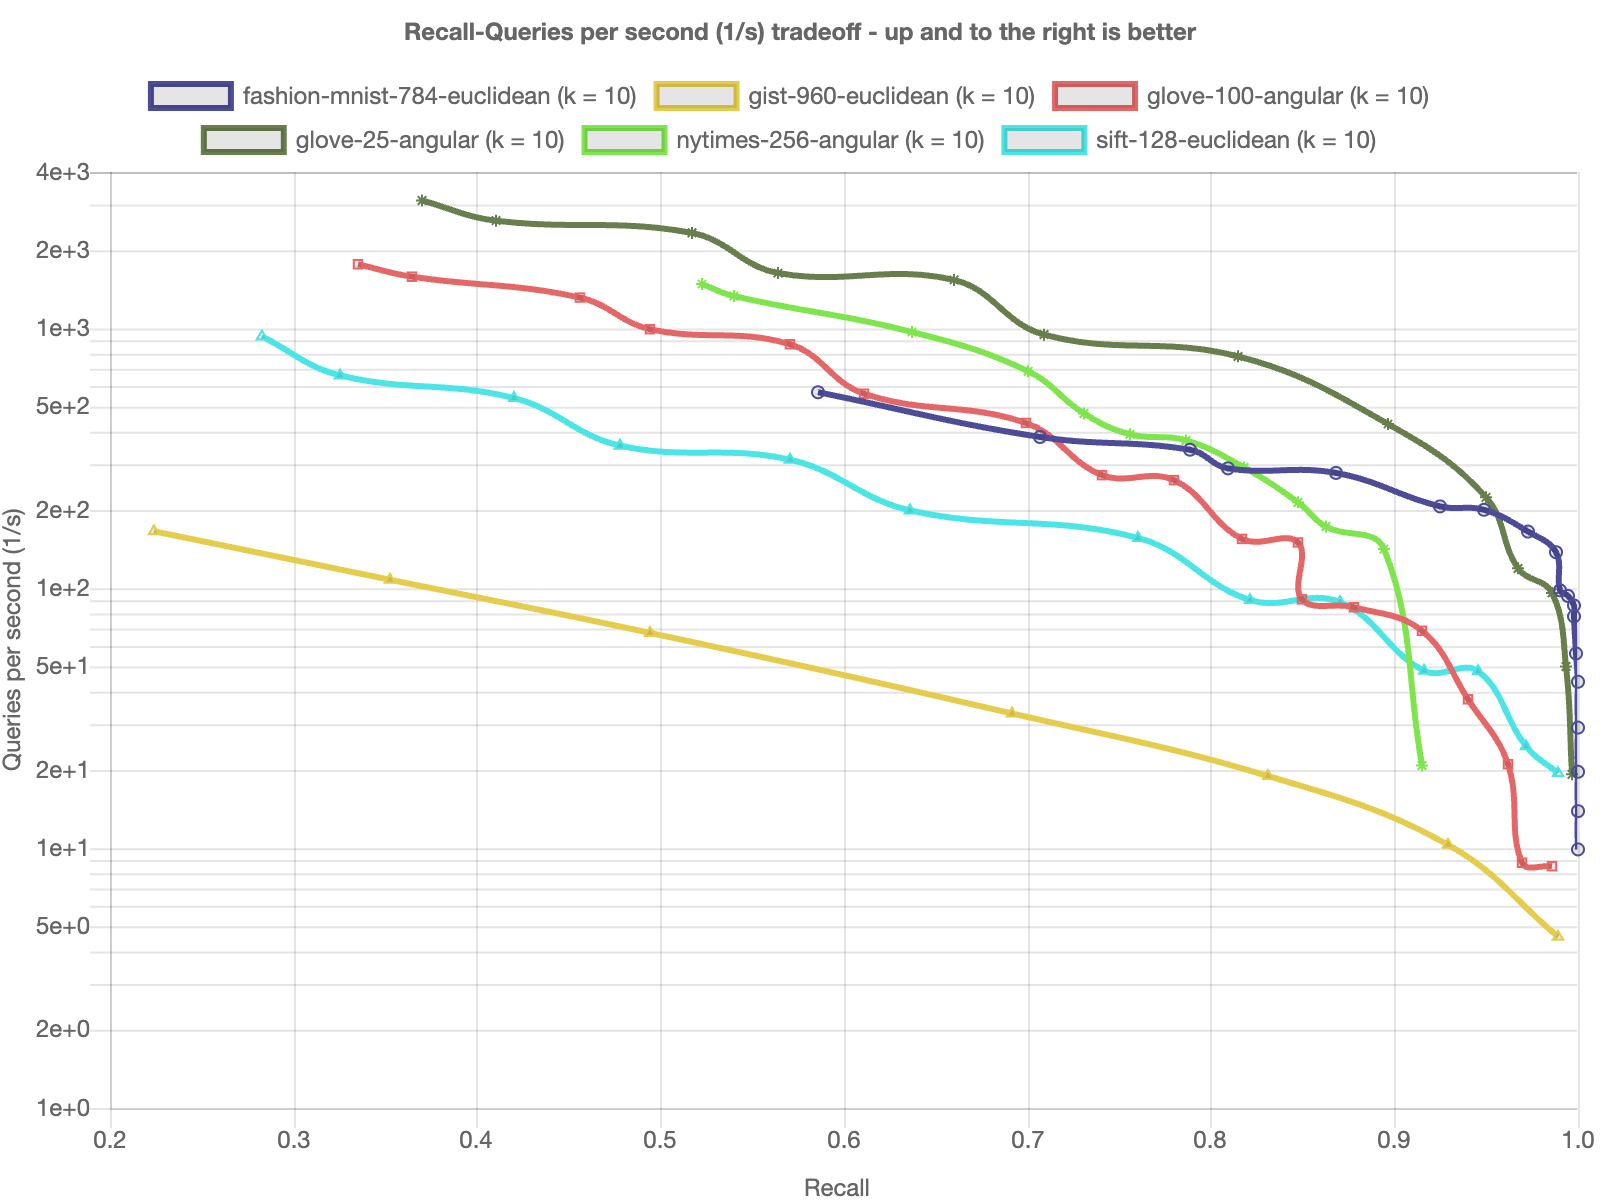
\includegraphics[width=0.85\linewidth]{images/pgvector.png}
    \caption{Recall-Queries-per-second-Tradeoff von pgvector über verschiedene 
             Benchmark-Datensätze \cite{pgvectorPlots}}
    \label{fig:ann_recall}
\end{figure}

Zudem ist der $vector$-Typ beim Einsatz von Indizes auf 2.000 Dimensionen begrenzt 
\cite{githubGitHubPgvectorpgvector}, was bei leistungsstarken Embedding-Modellen 
mit höherer Dimensionalität eine Einschränkung darstellen kann. Der erhöhte 
Speicherbedarf und die längeren Aufbauzeiten des HNSW-Index 
\cite{githubGitHubPgvectorpgvector} fallen im Kontext dieser Arbeit jedoch kaum 
ins Gewicht, da die verarbeiteten Log-Datensätze überschaubar sind und das 
eingesetzte Modell lediglich 384 Dimensionen erzeugt.

\paragraph{Fazit}
Die Wahl von PostgreSQL mit pg\_vector stellt damit eine pragmatische Entscheidung 
dar: Sie erfüllt alle definierten Anforderungen mit geringem Betriebsaufwand, auch 
wenn dedizierte Vektordatenbanken bei reinen Vektoroperationen im großen Maßstab 
performanter wären. Tabelle~\ref{tab:vektordatenbanken} fasst die Evaluation der 
drei Kandidaten anhand der definierten Anforderungen zusammen.

\begin{table}[h]
    \centering
    \begin{tabular}{lccc}
        \hline
        \textbf{Kriterium} & \textbf{Qdrant} & \textbf{Milvus} & 
        \textbf{PostgreSQL + pg\_vector} \\
        \hline
        Schwellwert-basierte Suche & $\times$ & $\times$ & \checkmark \\
        Metadatenspeicherung       & \checkmark & \checkmark & \checkmark \\
        On-Premises-Betrieb        & \checkmark & \checkmark & \checkmark \\
        \hline
    \end{tabular}
    \caption{Vergleich der evaluierten Vektordatenbanken anhand der 
             Auswahlkriterien}
    \label{tab:vektordatenbanken}
\end{table}


% Milvus\footnote{Offizielle Seite von Milvus: https://milvus.io/} ist eine weitere Open-Source-Datenbank für das Handling von Vektoren. Sie lässt sich On-Premises installieren und speichert Metadaten zusammen mit den Vektoren. Bei Abfragen von Vektoren begrenzt jedoch auch hier eine maximale Anzahl von Ergebnissen die Ausgabe, ähnlich wie bei Qdrant \footnote{Hier ist die Dokumentation der Query API von Milvus: https://milvus.io/docs/single-vector-search.md}.
% Da PostgreSQL in Kombination mit pg\_vector alle drei Kriterien erfüllt, fällt die Wahl auf diese Datenbank.


\section{Ähnlichkeitsmetriken: Kosinus-Ähnlichkeit im Vektorvergleich}
Die Erweiterung pg\_vector bietet mehrere Ähnlichkeitsmetriken, darunter die Kosinus-Ähnlichkeit und das Skalarprodukt.
Das Skalarprodukt vergleicht die Länge zweier Vektoren und stellt so eine Ähnlichkeit zwischen ihnen fest (siehe Abb. \ref{fig:skalar}) \cite{pineconeVectorSimilarity}.
\begin{equation}
  \bold{a} \cdot \bold{b} = |\bold{a}||\bold{b}|\cos{\alpha}
\end{equation}

\begin{figure}
    \centering
    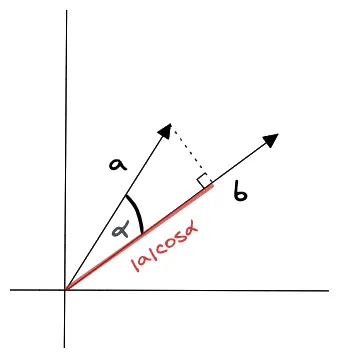
\includegraphics[width=0.5\linewidth]{images/b2af046e6a6d5d2057f2328171d0bdeba0489a90-338x357.png}
    \caption{Skalarprodukt zweier Vektoren}
    \label{fig:skalar}
\end{figure}

Die Kosinus-Ähnlichkeit (siehe Formel \ref{cos}) betrachtet hingegen nicht die Länge der Vektoren, sondern nur den Winkel zueinander \cite{pineconeVectorSimilarity}.
\begin{equation}
  sim(\bold{a},\bold{b}) = \frac{\bold{a}\cdot \bold{b}}{||\bold{a}||\cdot||\bold{b}||}
  \label{cos}
\end{equation}
Bei der Auswahl der Ähnlichkeitsmetrik ist die Vorverarbeitung relevant: Wenn ein Modell den Text vektorisiert, das beispielsweise die Kosinus-Ähnlichkeit nutzt, ist es von Vorteil, diese Metrik auch beim Vergleich der Vektoren zu verwenden \cite{pineconeVectorSimilarity}. In diesem Fall kommt das Embedding-Modell „sentence-transformers/all-MiniLM-L6-v2“ zum Einsatz, bei dessen Training auch die Kosinus-Ähnlichkeit Verwendung fand \footnote{Mehr Details unter Training procedure: https://huggingface.co/sentence-transformers/all-MiniLM-L6-v2}.

\section{Entwurf eines iterativen Algorithmus zur Vektorgruppierung}\label{PG_Algorithmn}
Nach der Datenbankwahl folgt der Entwurf eines Algorithmus zur kontinuierlichen Gruppierung der Lognachrichten mithilfe der Vektordatenbank. Diese Vorgehensweise wurde während der Praxisphase entworfen und praktisch eingesetzt. Der Algorithmus verarbeitet eingehende Lognachrichten sequenziell und vergleicht jede einzeln mit den bereits bestehenden Cluster-Schwerpunkten, unabhängig davon, ob zu diesem Zeitpunkt bereits Cluster existieren. Eine Unterscheidung zwischen einer initialen Gruppierung beim ersten Start und einer nachträglichen Erweiterung bestehender Cluster ist dadurch nicht erforderlich: Liegt noch kein Cluster-Schwerpunkt innerhalb des Schwellwerts vor, kann keine Ähnlichkeit gefunden werden, sodass automatisch ein neuer Cluster entsteht. Kaltstart und fortlaufender Betrieb werden so durch denselben Mechanismus abgedeckt.

Listing~\ref{lst:cluster-batch} zeigt den Pseudocode des Verfahrens.

\begin{minted}[linenos, breaklines, fontsize=\small]{python}
def cluster_batch(logs, embeddings, schwellwert):
    cluster_anzahl = aktuelle_cluster_anzahl()

    # Schritt 1: neue Logs mit ihren Embeddings persistieren
    for log, embedding in zip(logs, embeddings):
        speichere_log(log, embedding, verarbeitet=False)

    unverarbeitete_logs = hole_unverarbeitete_logs()  # aufsteigend nach id

    # Schritt 2: jedes Log einzeln und sequenziell zuordnen
    for log in unverarbeitete_logs:
        gefundener_cluster = finde_naechsten_cluster(log.embedding, schwellwert)

        if gefundener_cluster is not None:
            cluster_id = gefundener_cluster.id
        else:
            cluster_anzahl += 1
            cluster_id = cluster_anzahl

        weise_zu_und_markiere_verarbeitet(log, cluster_id)

        # Schritt 3: betroffenen Cluster-Schwerpunkt sofort aktualisieren
        aktualisiere_durchschnittsvektor(cluster_id)

    return alle_cluster_zuweisungen()
\end{minted}
\captionof{lstlisting}{Iteratives Clustering neu eingehender Lognachrichten (Pseudocode)}
\label{lst:cluster-batch}

Schritt 1 persistiert alle neu eingehenden Lognachrichten zusammen mit ihrem Embedding-Vektor und markiert sie als unverarbeitet. Schritt 2 iteriert anschließend über alle unverarbeiteten Logs in der Reihenfolge ihres Eintreffens und sucht für jedes Log mittels einer Schwellwert-Suche über die Kosinus-Distanz den nächstgelegenen Cluster-Schwerpunkt. Liegt ein Schwerpunkt innerhalb des Schwellwerts~$\tau$, wird das Log dem zugehörigen Cluster zugewiesen; andernfalls eröffnet das Verfahren einen neuen Cluster mit fortlaufender Nummer. In Schritt 3 wird unmittelbar nach jeder Zuweisung der Durchschnittsvektor (\texttt{avg\_embedding}) des betroffenen Clusters neu berechnet, sodass nachfolgende Logs im selben Durchlauf bereits gegen den aktualisierten Schwerpunkt geprüft werden. Der Vergleich mit den Cluster-Schwerpunkten bildet dabei die alleinige Zuordnungsstrategie des Verfahrens.

Aus der sequenziellen Verarbeitung folgt eine inhärente Reihenfolgeabhängigkeit: Welche Lognachricht zuerst einen Cluster-Schwerpunkt definiert, beeinflusst, welchem Cluster ähnliche nachfolgende Logs zugeordnet werden. Bei unterschiedlicher Eingangsreihenfolge derselben Lognachrichten entstehen folglich potenziell abweichende Clusterzuordnungen. Dieser Effekt ist typisch für inkrementelle Online-Verfahren und wird in Kapitel~\ref{chap:eval} bei der Bewertung der Reihenfolge-Stabilität wieder aufgegriffen.
